\documentclass[12pt]{article}

 %%%
 \usepackage[utf8]{inputenc}
 \usepackage{graphicx}
 \usepackage{xcolor}
 \usepackage{geometry}\geometry{a4paper, total={170mm,257mm}, left=20mm, top=20mm}

 \definecolor{PIKorange}{RGB}{227, 114, 34}
 \definecolor{PIKgray}{RGB}{142, 144, 143}

 \title{ \bfseries \color{PIKorange} Antilles: information on national emissions, population and GDP, and mitigation targets}

 %%%

 \begin{document}

 \maketitle

 %%%
 \noindent \textbf{Authors:} \newline
 \indent Annika Guenther$^{1}$ \newline
 \indent Johannes Guetschow$^{1}$ \newline
 \noindent \textbf{Affiliations:} \newline
 \indent 1. Potsdam Institute for Climate Impact Research, Germany \newline
 \noindent \textbf{DOI:} [to be added] \newline

 \textbf{TODO}
 \begin{itemize}
 \item Table with info on target (main and reclass; emissions from NDC; target quantis + plot).
 \item GWP: NDC emissions coverted from AR2 to AR4 by national conversion factor (2010--2017, PRIMAP-hist v2.1).
 \item References!
 \end{itemize}

 %%%
 \section{Non-LULUCF emissions and socio-economic data}
 \label{sec:nonLULUCFSocioEco}
 With national emissions of 7.5~Mt CO$_2$eq, Antilles contributed 0.01\% to global emissions in 2017, and in 2030 its share is estimated to stay at a similar level (Table~\ref{tab:overview}).
 The estimates for 2030 are based on the downscaled SSP2\footnote{\textbf{SSPs}: Shared Socio-economic Pathways.
 Narratives and challenges to mitigation and adaptation: 
 SSP1: Sustainability, Taking the Green Road (low~/ low);
 SSP2: Middle of the Road (medium~/ medium);
 SSP3: Regional Rivalry, A Rocky Road (high~/ high);
 SSP4: Inequality, A Road Divided (low~/ high); and
 SSP5: Fossio-fuelled Development, Taking the Highway (high~/ low).} Middle of the Road marker scenario (dmSSP2), in which Antilles is estimated to emit 7.2~Mt CO$_2$eq in 2030.
 That change in emissions would constitute a decrease of -3.7\% compared to 2017. 
 The pathways dmSSP1--5 show a range of 7.2--7.2~Mt CO$_2$eq in 2030, and 7.2--7.2~Mt CO$_2$eq in 2050.
 The country's global rank in terms of total emissions per unit of GDP\footnote{\textbf{GDP}: Gross Domestic Product. 
 Throughout this document the GDP is given as GDP~PPP, with PPP being the Purchasing Power Parity.} was 8 in 2017, and 4 regarding the per-capita emissions (5 and 4 in 2030).
 In terms of accumulated historical emissions, Antilles contributed to the global 1850--2017 emissions by 0.07\%. 
 When only accounting for the years 1990--2017, its contribution decreases to 0.01\%.
 All of the emissions are presented following GWP~AR4\footnote{\textbf{Global Warming Potential (GWP)}: we use GWP values from the IPCC 4$^{th}$ Assessment Report (AR4). 
 They reflect the forcing potential of one kilogram of a gas' emissions in comparison to one kilogram of CO$_2$ (GWP$_{CO2}$ = 1). 
 The GWPs correspond to a 100-yr period and are for CH$_4$:~25, for N$_2$O:~298, for SF$_6$:~22800, and for NF$_3$:~17200. 
 For the basket of HFC-gases the GWPs from AR4 are in the range 4--14800, and for PFCs 7190--12200. 
 To assess emissions of several GHGs, their emissions are weighted by their respective GWPs and presented in CO$_2$ equivalents (CO$_2$eq).}, and exclude emissions from LULUCF\footnote{\textbf{LULUCF}: Land Use, Land-Use Change and Forestry. 
 Emissions from LULUCF are excluded throughout the document, unless stated otherwise.} (exclLU), and bunkers fuels\footnote{\textbf{Bunkers fuels}: emissions from international aviation and shipping.} emissions (exclBunkers).
 \begin{table}[htbp]
 \centering
 \caption{National emissions (dmSSP2), GDP and population for Antilles, together with the emissions per unit of GDP and per capita emissions (all for 2017 and 2030). 
 Additionally, the global share and its rank are displayed.}
 \label{tab:overview}
 \begin{tabular}{l || l r l r r}
 \bfseries  & \bfseries Year & \bfseries Total & \bfseries Unit & \bfseries Glob. share & \bfseries Rank \tabularnewline \hline \hline
 \bfseries Emissions & 2017 & 7.5 & Mt CO$_2$eq & 0.01\% & 151 \tabularnewline 
 \bfseries  & 2030 & 7.2 & Mt CO$_2$eq & 0.01\% & 154 \tabularnewline \hline
 \bfseries GDP & 2017 & 5.1 & Billion 2011~GK\$ & 0.004\% & 166 \tabularnewline 
 \bfseries  & 2030 & 5.3 & Billion 2011~GK\$ & 0.002\% & 173 \tabularnewline \hline
 \bfseries Emissions & 2017 & 1.5 & t CO$_2$eq / Thousand 2011~GK\$ & 1.3\% & 8 \tabularnewline 
 \bfseries per GDP & 2030 & 1.4 & t CO$_2$eq / Thousand 2011~GK\$ & 1.8\% & 5 \tabularnewline \hline
 \bfseries Population & 2017 & 228.8 & Thousand Pers & 0.003\% & 177 \tabularnewline 
 \bfseries  & 2030 & 222.2 & Thousand Pers & 0.002\% & 177 \tabularnewline \hline
 \bfseries Emissions & 2017 & 32.7 & t CO$_2$eq /  Pers & 2.2\% & 4 \tabularnewline 
 \bfseries per capita & 2030 & 32.5 & t CO$_2$eq /  Pers & 2.2\% & 4 \tabularnewline 
 \end{tabular}
 \end{table}

 For Antilles, in 2017 the main emissions share on sectoral level (Fig.~\ref{fig:tsEmi}) came from the Energy sector (97.7\%), followed by IPPU (1.5\%), and Other (0.6\%). 
 The Kyoto~GHG\footnote{\textbf{Kyoto~GHG} (Greenhouse Gas) basket: carbon dioxide (CO$_2$), methane (CH$_4$), nitrous oxide (N$_2$O), hydrofluorocarbons (HFCs), perfluorocarbons (PFCs), sulfur hexafluoride (SF$_6$), and nitrogen trifluoride (NF$_3$).} with the highest emissions in 2017 was CO$_2$, constituting as much as 98.2\% of the national emissions. 
 Second largest contributor was CH$_4$ (0.9\%), followed by N$_2$O (0.9\%). 
 The total of F-gases\footnote{\textbf{F-gases} (fluorinated gases): basket of HFCs, PFCs, and the gases SF$_6$ and NF$_3$. 
 Some F-gases have very long atmospheric lifetimes and high Global Warming Potentials.} only represented 0.0\%.
 The total CO$_2$ emissions are expected to be 98.1\% of the national Kyoto~GHG emissions in 2030 (dmSSP2).
 \begin{figure}[htbp]
 \centering
 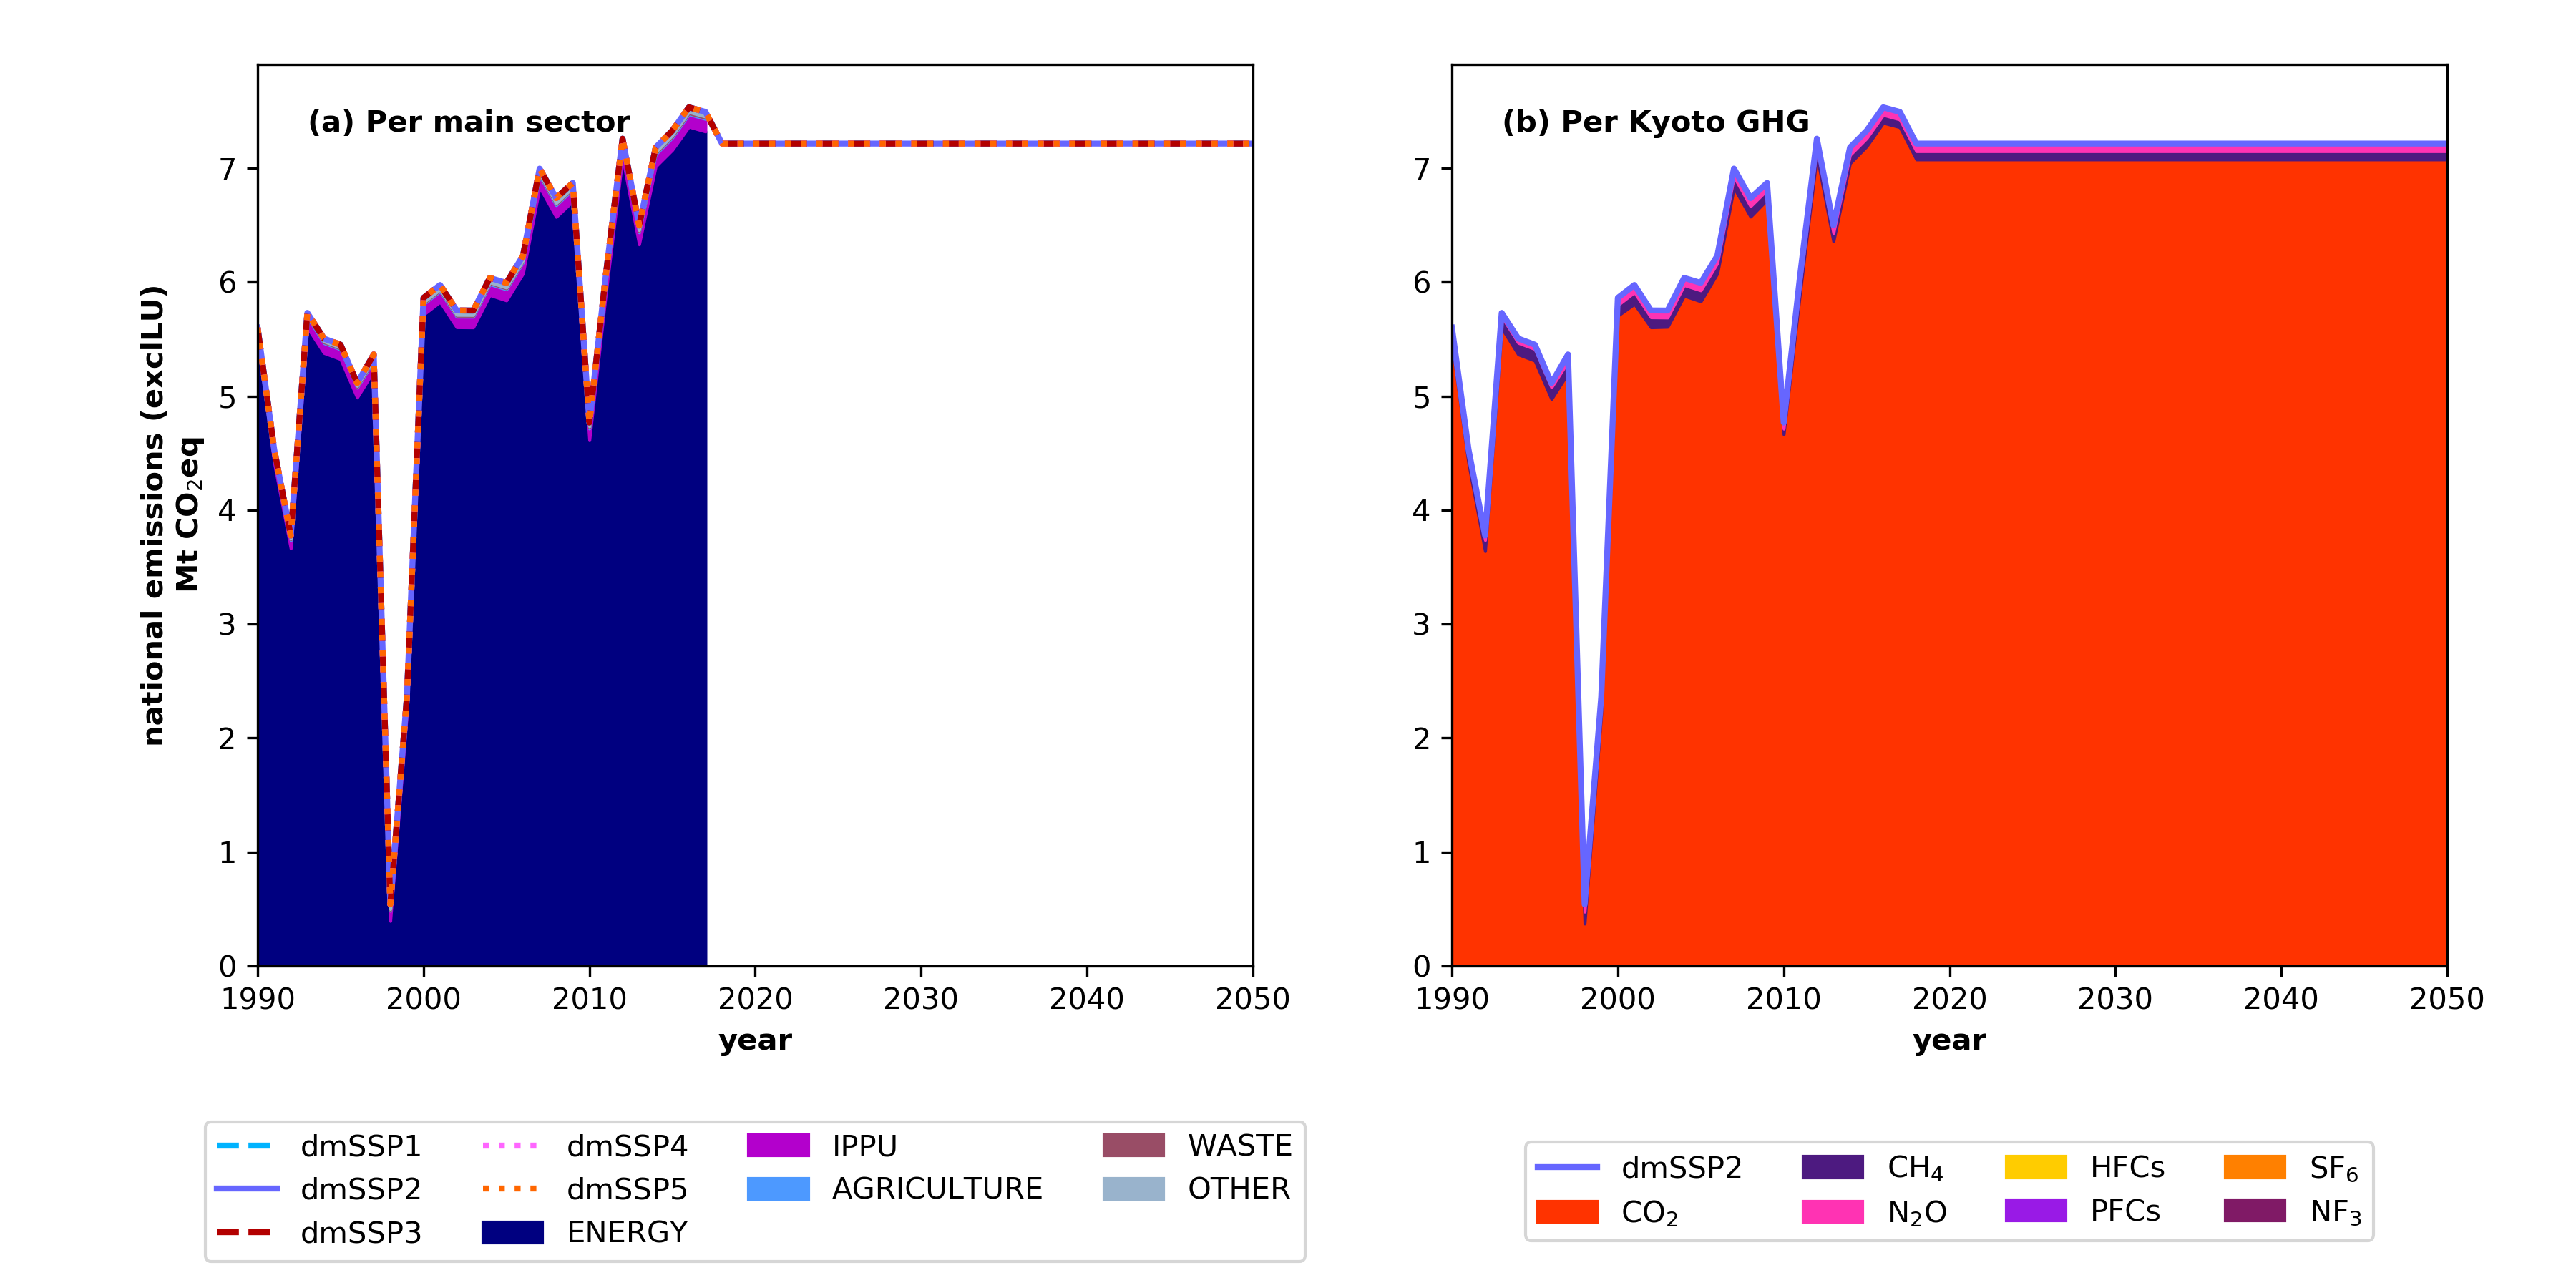
\includegraphics[width=\textwidth]{C:/Users/annikag/primap/ndc_quantifications/latex_files/ANT/ts_emi_exclLU_ANT.png}
 \caption{'Stacked' timeseries of national emissions (exclLU) per main-sector (a) and Kyoto~GHG (b). 
 No information available on the sectoral contributions after 2017.}
 \label{fig:tsEmi}
 \end{figure}
 \begin{figure}[htbp]
 \centering
 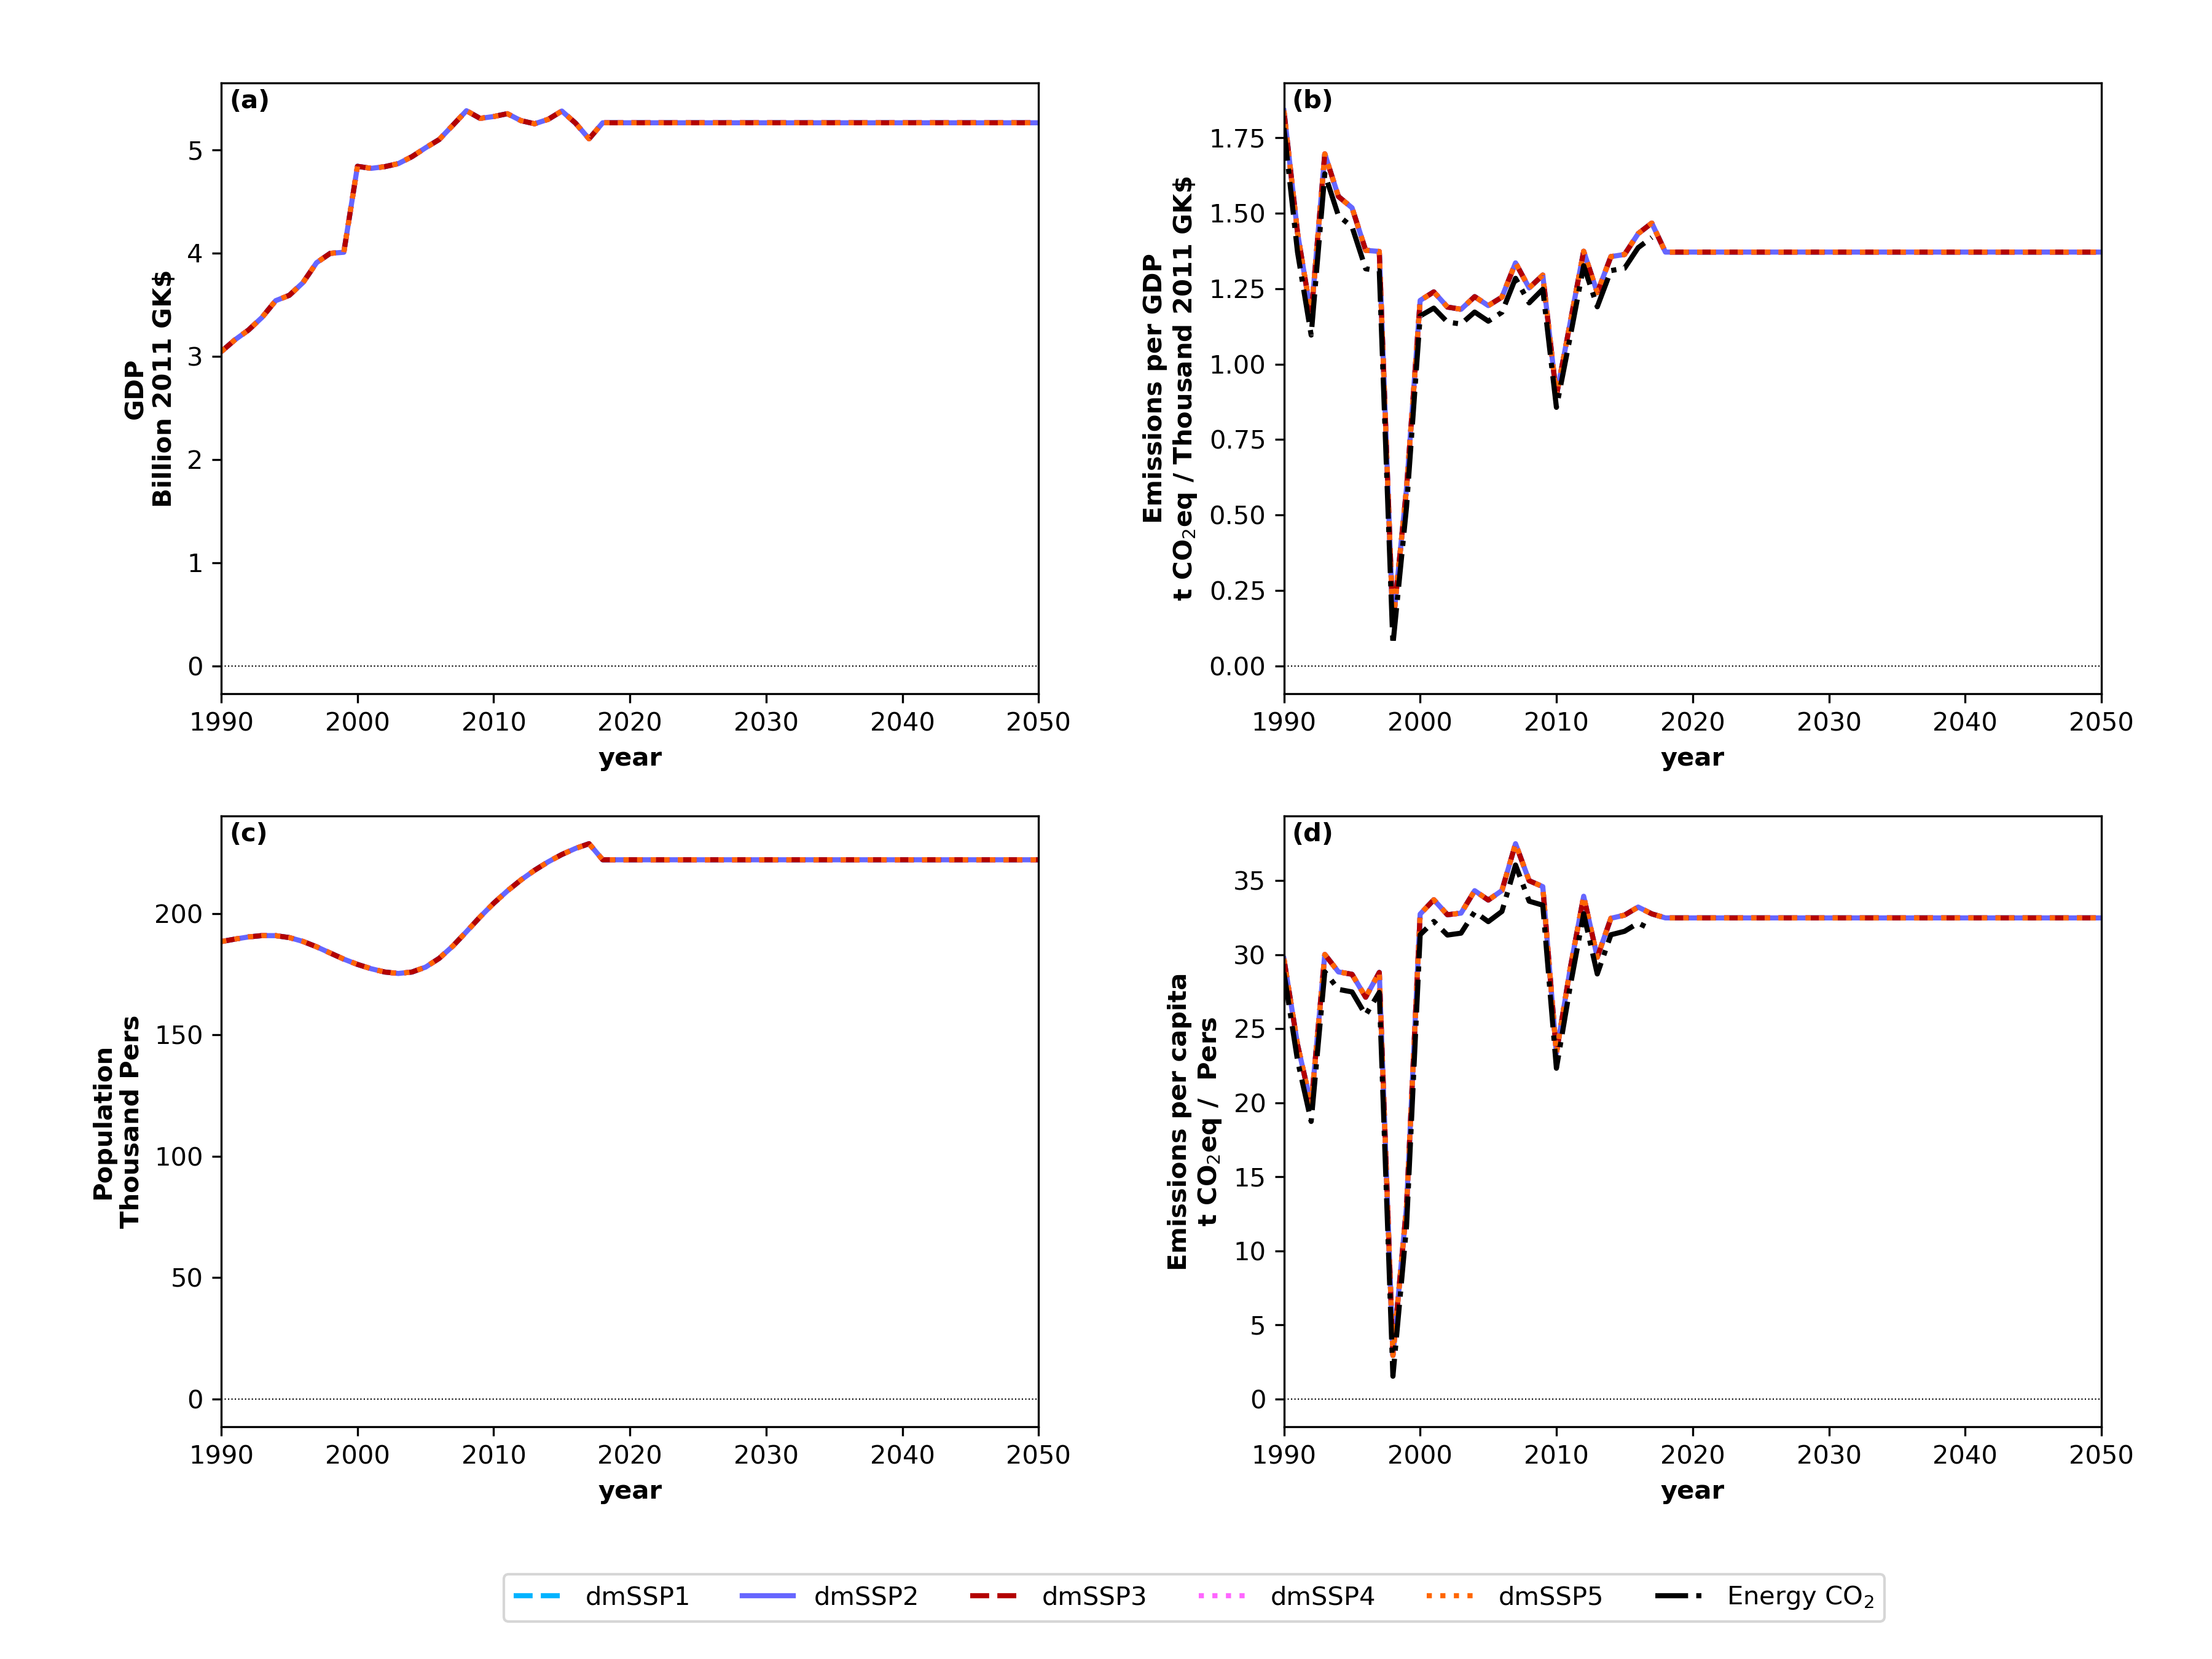
\includegraphics[width=\textwidth]{C:/Users/annikag/primap/ndc_quantifications/latex_files/ANT/ts_gdp_pop_ANT.png}
 \caption{Timeseries of national GDP (a) and population (c), and Kyoto~GHG emissions (exclLU, exclBunkers) per unit of GDP (b) or per capita (d).}
 \label{fig:tsSocioEco}
 \end{figure}

 The national GDP decreased in recent years, and the emissions per unit of GDP had a similar trend (Fig.~\ref{fig:tsSocioEco}).
 The population increased, and the per capita emissions were on the rise. 
 Following dmSSP2, the GDP is projected to increase after 2017 but to drop again before 2050. 
 The emissions per GDP are estimated to decrease towars 2050. 
 Antilles's population is assumed to diminish towars 2050, and the per capita emissions are expected to decline towars 2050. 

 %%%
 \section{LULUCF emissions}
 \label{sec:emiLULUCF}
 LULUCF emissions data for Antilles are available from the following sources (Fig.~\ref{fig:tsLULUCF}): FAO (2019).

 \textbf{High fluctuations? Data gaps? Difference between sources?}
 \begin{figure}[htbp]
 \centering
 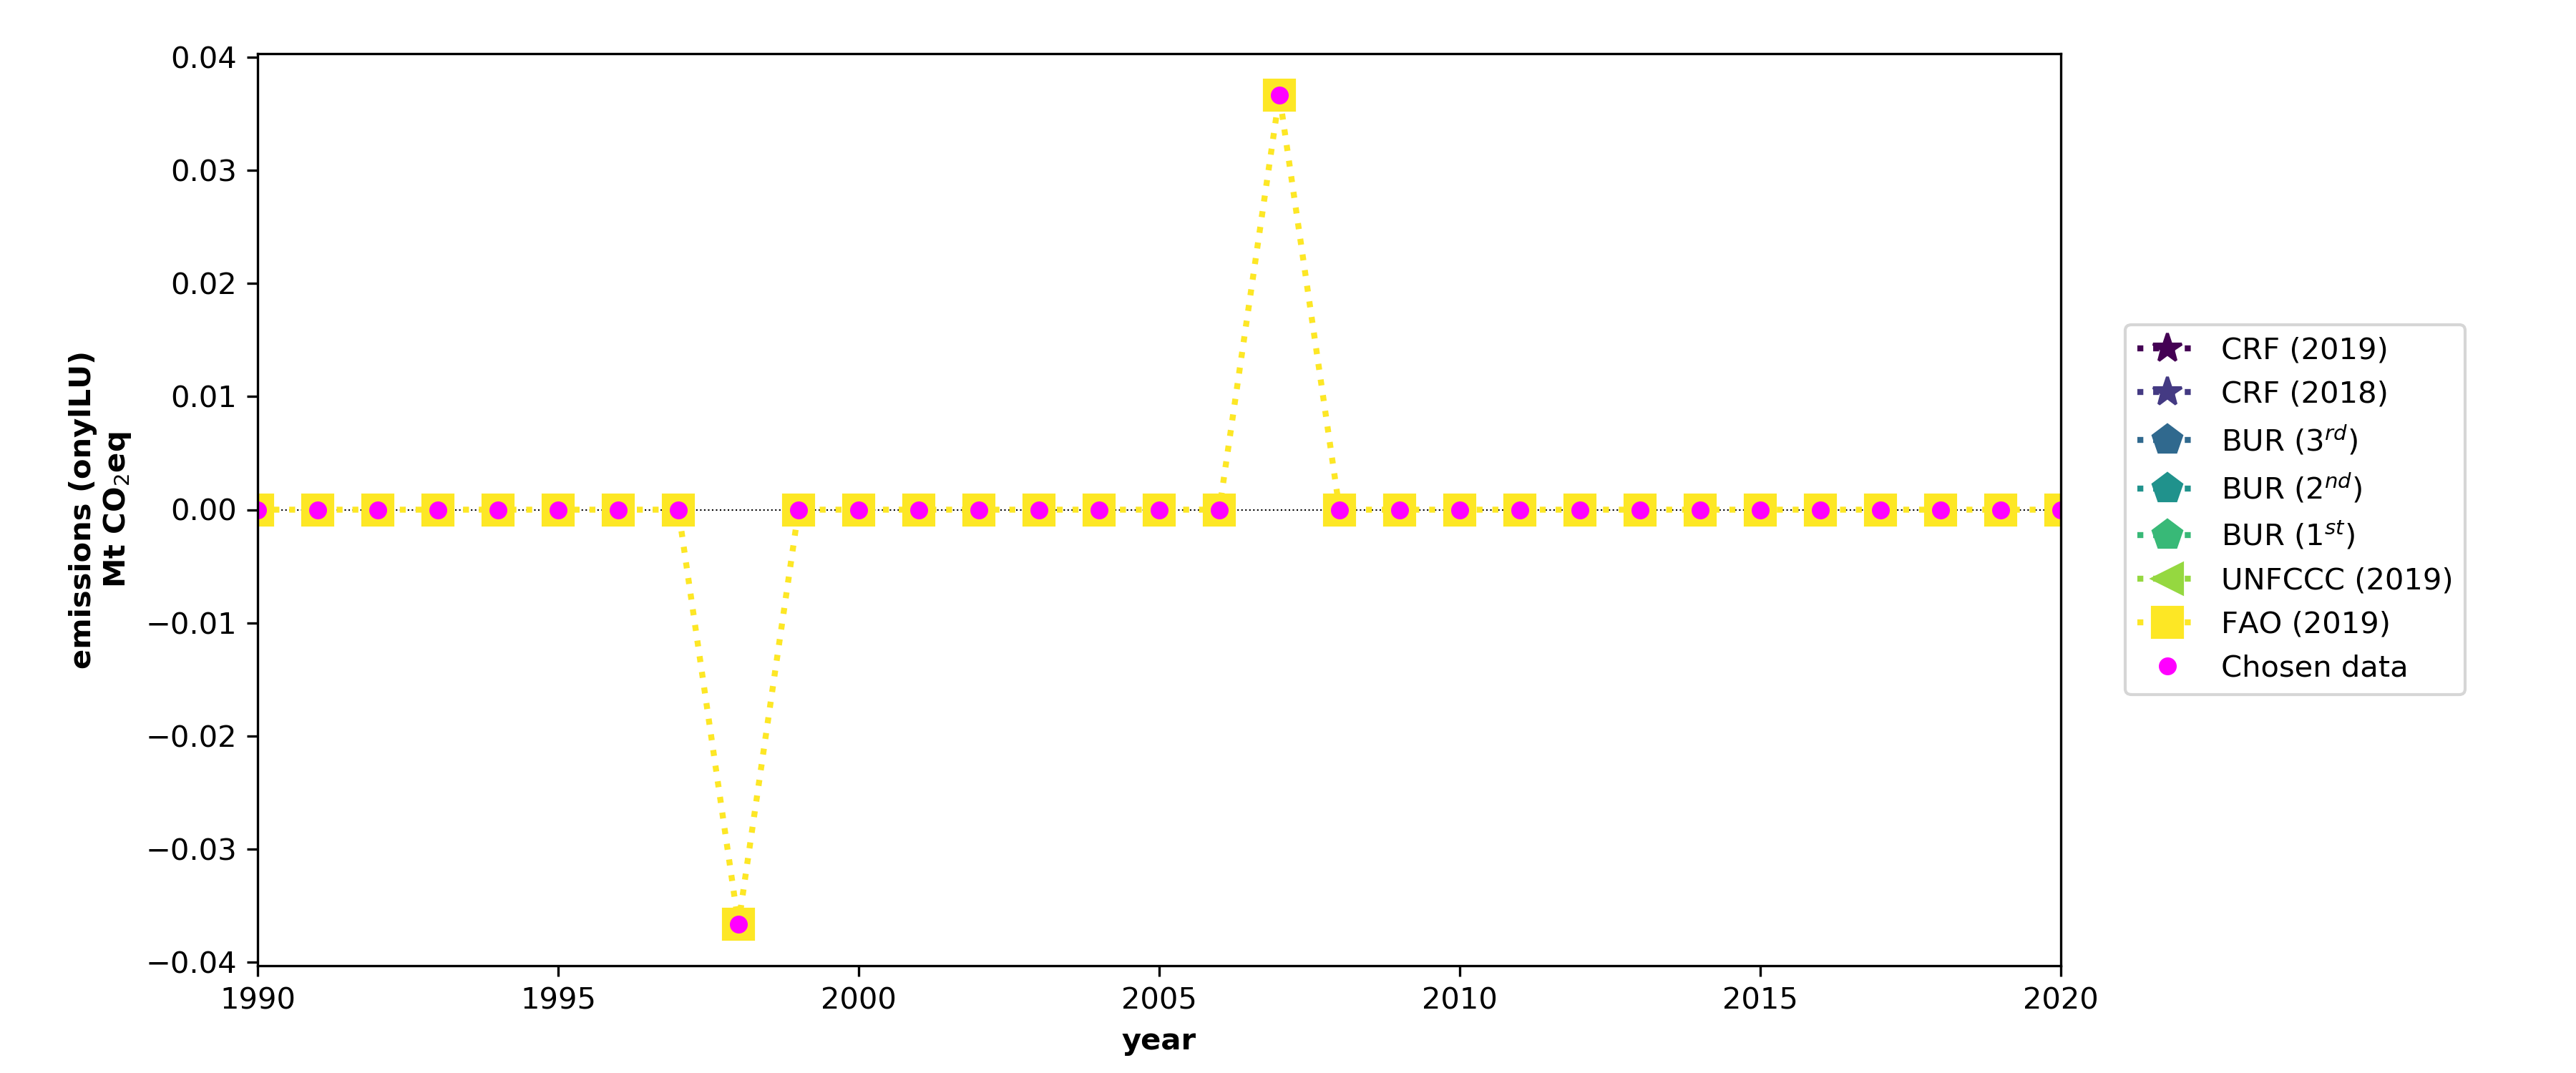
\includegraphics[width=\textwidth]{C:/Users/annikag/primap/ndc_quantifications/latex_files/ANT/ts_emi_onlyLU_ANT.png}
 \caption{Timeseries of emissions from LULUCF (CO$_2$ plus CH$_4$ and N$_2$O) as available from different data-sources. 
 Indicated in pink are the 'chosen' data, as used in our assessment of Antilles's NDC (if needed). 
 The pink timeseries was inter- and~/ or extrapolated (interpolation: linear, extrapolation: constant).}
 \label{fig:tsLULUCF}
 \end{figure}

 %%%
 \section{Mitigation targets (NDC)}
 \label{sec:mitiTars}

 \textbf{ 
 Give the \%cov for the base and target year (and 2017).
 Global share for 2030 for the mitigated pathways and \% reduction relative to 1990 and 2017.
 Table with the 'input' data and the resulting targets (like ndcs\_targets.csv).}
 Antilles does not have an (I)NDC.
 Therefore the assumed 'mitigated' emissions pathways used for global aggregates equal the baseline emissions (dmSSP1--5).

 %%%
 \section{Data sources and references}
 \label{sec:dataSourcesRefs}
 PRIMAP-hist v2.1: emissions from PRIMAP-hist are data from the country reported data priority scenario (HISTCR).

 %%%
 \end{document}
